\section{The CnC Programming Model}
\label{sec:cnc}

The Concurrent Collections Programming Model (CnC), developed by
Intel, is one such data-centric programming model. Its deterministic
% RRL: "task-based" vs. "data-centric" -- choose one
semantics allow a task-based runtime to programmatically exploit
parallelism. In addition, it allows for a secondary file, called a
tuning spec, to provide additional hints to improve performance.

\begin{figure}[t!]
  \centering
  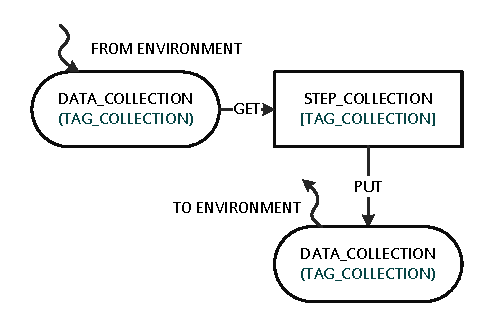
\includegraphics[width=0.5\textwidth]{drawings/CnCExample.pdf}
  \caption{CnC Graph Semantics}
  \label{fig:cnc_graph}
\end{figure}

The CnC model can be thought of as a producer-consumer paradigm where
data is produced and consumed by tasks, or ``steps'' in CnC
terminology. The produced and consumed data is declared explicitly in
an input file, known as a ``graph file''. The steps themselves are
also entities that can be produced. When a step produces another step,
this is known as a ``control dependency'' and is also declared in the
graph file.

Figure~\ref{fig:cnc_graph} shows a graph file. The rectanglees are
``step collections'', the ``data collections'' are ovals, and the
dependencies are directed edges between them. The title of a step
collection is usually a descriptive verb and the title of a data
collection is usually a descriptive noun. The control dependencies are
not shown. A text description of Figure~\ref{fig:cnc_graph} (which
includes control information) is provided to CnC when designing a CnC
application.
% RRL: "designing", not "running"?
Section~\ref{sec:raytracing} shows an example of this.

By declaring all dependencies between steps and data, the specifics
regarding how the algorithm is executed is abstracted out of the
implementation. For example: It is clear what data is needed by a
given step, so if that data has not been produced yet, the step will
not be scheduled. This allows the runtime to optimally decide when and
where to schedule computation. By way of contrast, in a conventional
multithreaded program, it is the responsibility of the programmer to
guarantee that a thread's inputs are available and consequently start
the thread.

For some more complicated semantics, additional hints can be provided
to the runtime through a ``tuning specification''. As the tuning
specification usually is in a separate file, this makes it easy to run
the same program on different architectures, as no rewrites of the
application are necessary to switch platforms: just the tuning
specification.

\subsection{Language Specifics}
The CnC model is built on three key constructs; step collections, data
collections, and control collections ~\cite{budimlicconcurrent}. A
step collection defines computation, an instance of which consumes and
produces data. The consumed and produced data items belong to data
collections. Data items within a data collection are indexed using
item ``tags'': tuples that, like primary keys, can uniquely identify a
data item in the data collection. Finally, the control collection
describes the prescription, or creation, of step instances. The
relationship between these collections as well as the collections
themselves are defined in the graph file.

Developing a CnC application then begins with designing the graph
file. An algorithm is broken down into computation steps, instances of
which correspond to different input arguments. These steps, along with
the data collections become nodes, in the graph. Each step can
optionally consume data, produce data, and/or prescribe additional
computation. These relationships: producer, consumer, and control,
define the edges of the graph and will dynamically be satisfied as the
program executes.

The next and final required step in producing a CnC application is to
implement the step logic. The flow within a single step is: consume,
compute, and produce. This ordering is required as there is no
guarantee the data a step needs will be ready when the step begins
executing. This is due to steps being preemptively scheduled when they
are prescribed. Most of the time the data \emph{will} be ready when a
step begins execution, but occasionally and often due to an
implementation error, a step’s data may never be available.
Internally, if the data is not ready when a step begins execution
it will halt execution and try again later. To improve performance,
hints can be provided through the tuning specification to increase the
likelihood that steps are schedule for execution when their required
input data is ready.

\subsection{Example}

\begin{figure}[!tb]
  \centering
  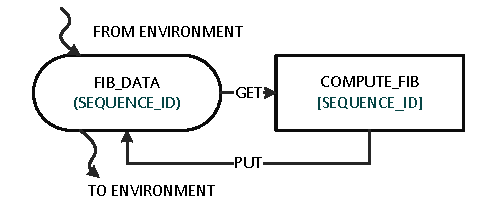
\includegraphics[width=0.5\textwidth]{drawings/FibExample.pdf}
  \caption{A CnC Graph to Compute the Fibonacci Sequence}
  \label{fig:fib_graph}
\end{figure}

% apparently putting this here makes it show up on the top of page 3, where I want it
\begin{figure*}[t]
  \centering
  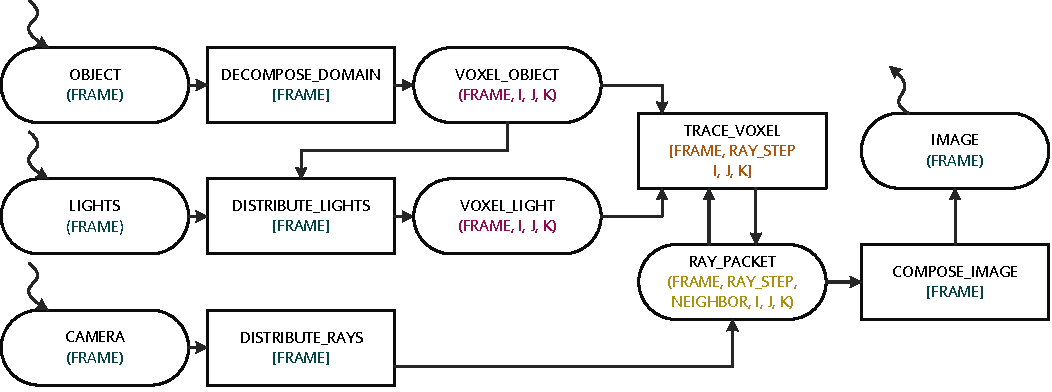
\includegraphics[width=\textwidth]{drawings/CnC.pdf}
  \caption{CnC Graph}
  \label{fig:cnc}
\end{figure*}

Figure~\ref{fig:fib_graph} shows an example of a
simple iterative implementation of the Fibonacci sequence. This
application consists of one step, COMPUTE\_FIB, which takes the
previous two computed values as input and produces the next value in
the sequence. One data collection, FIB\_DATA, exists for the
application. Data within the collection is indexed by a tag consisting
of the sequence number. Tags 1-5, then index the values 1,
1, 2, 3, 5, respectively. The first two values of the data collection
are produced by the environment, the rest of the values in the
collection are produced as needed by COMPUTE\_FIB. A tag exists for
COMPUTE\_FIB as well. We can index this collection by the integer
sequence a particular instance will produce. For example, the step
% RRL: What do you mean by "integer sequence"? The *whole* Fibo sequence?
instance at tag 3 will consume the data at tag 1 and 2, and produce
data at tag 3. Specifically it will consume 1, 1 and produce 2.
The number of steps executed in this example is provided by the 
environment.

%%% Local Variables: 
%%% mode: latex
%%% TeX-master: "main"
%%% End: 
